% Драфт: Секция 3.3, обсуждение результатов MANGO
% Источник: parts/neurotrain/main.tex, строки 573–748 (Discussion + Appendix C)
% Статья: Pospelov2025, Neurocomputing

\subsection{Сравнение свойств селективности в импульсной и классической сети}\label{sec:mango_snn_vs_ann}

Для того чтобы оценить, в какой степени описанные выше закономерности определяются импульсной природой исследуемой сети, аналогичный анализ был проведён на стандартной (неимпульсной) ИНС архитектуры ResNet18 --- по сути, той же модели без импульсных слоёв. Методы оптимизации на основе разложения тензорного поезда были применены для выявления MEI нейронов всех 8 блоков ResNet18 на протяжении обучения; полученные данные подвергнуты тому же анализу, что и для импульсной сети. Результаты выявили существенные различия между двумя типами сетей (рис.~\ref{nt:ann_stats}).

\begin{figure}[ht]
\centering
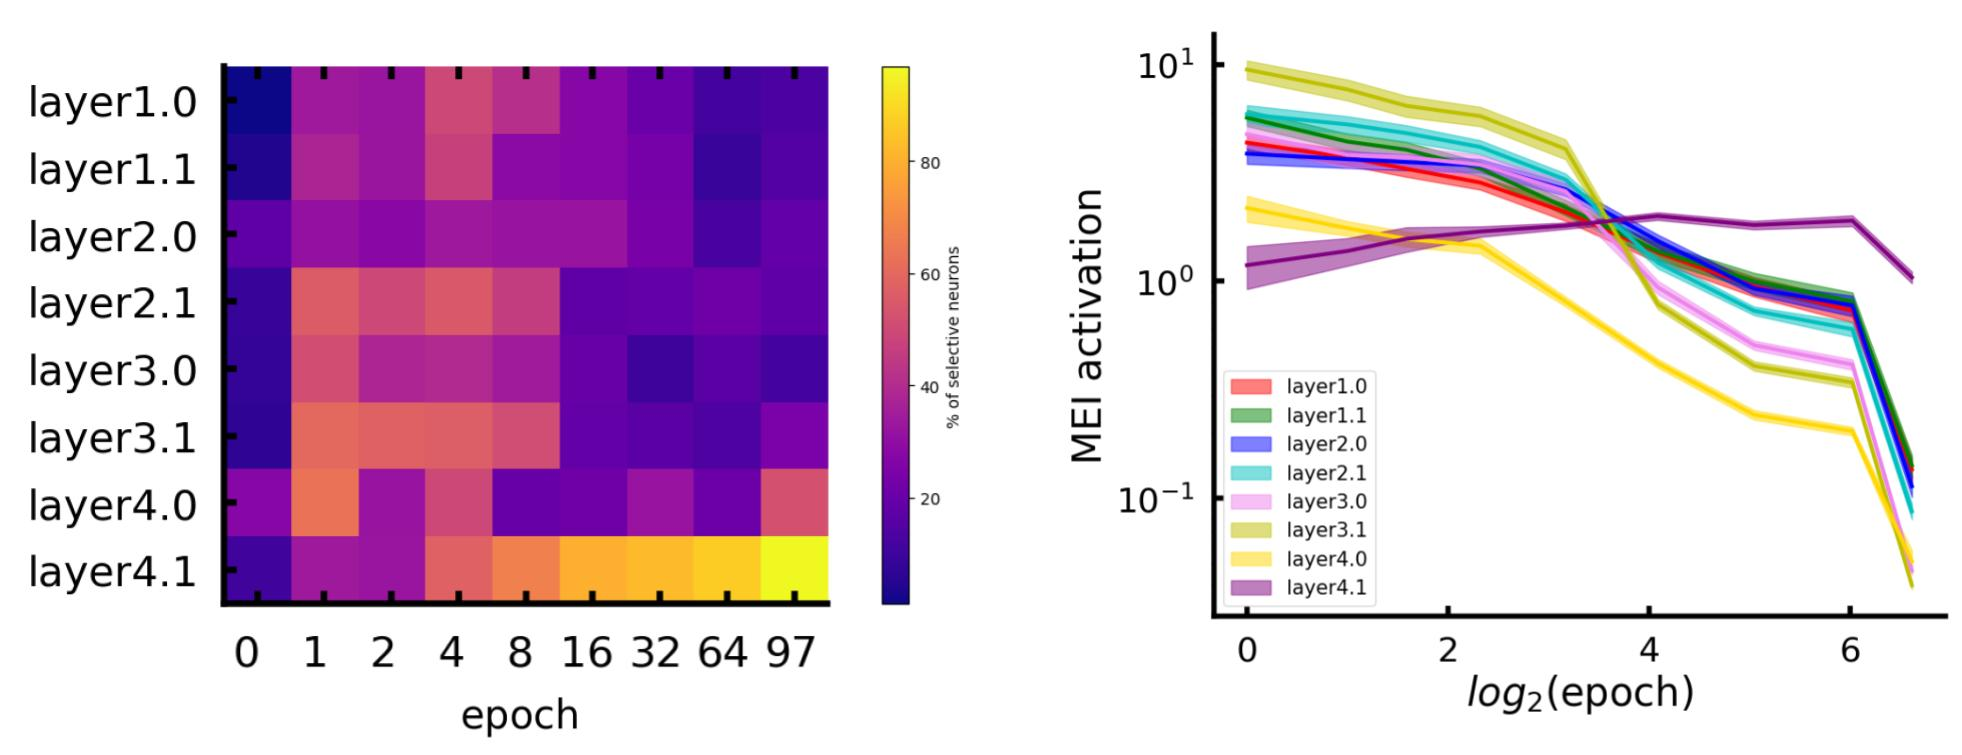
\includegraphics[width=0.95\textwidth]{images/neurotrain/a3.jpg}
\caption{\textbf{Слева:} доля класс-селективных нейронов в неимпульсной ИНС ResNet18. Горизонтальная ось~--- номер эпохи, вертикальная~--- слои (ниже~= глубже). \textbf{Справа:} MEI-связанные активации в неимпульсной ИНС по слоям во время обучения. Заштрихованные области~--- стандартные ошибки.}
\label{nt:ann_stats}
\end{figure}

Основные наблюдения таковы.

\begin{enumerate}
    \item \textbf{Динамика селективности.} В неимпульсной ИНС доля класс-селективных нейронов растёт или остаётся неизменной на протяжении обучения во всех слоях. В импульсной сети этот процесс имеет явно двухфазный характер: начальный рост доли селективных единиц сопровождается её снижением во всех слоях, кроме последнего, где она монотонно увеличивается (рис.~\ref{nt:ann_stats}, слева). Складывается впечатление, что селективность <<перетекает>> в последний слой, а оптимальные стимулы промежуточных слоёв становятся менее утончёнными.

    \item \textbf{Уверенность сети.} Уверенность классической ИНС (измеренная отрицательной энтропией выходов) при инференсе на сгенерированных MEI оказалась значительно ниже, чем в импульсной версии. Единственным слоем со стабильными и надёжными класс-связанными MEI был последний, преимущественно на поздних эпохах обучения.
\end{enumerate}

Эти различия допускают интерпретацию в контексте общей динамики обучения нейронных сетей. Показано, что забывание~--- распад информации, содержащейся в весах,~--- играет критическую роль в достижении инвариантности и разделения при обучении представлений~\cite{critical-learning-periods}. Этим может объясняться снижение селективности и амплитуд активации в промежуточных слоях. Одновременно вычислительная роль последних слоёв возрастает, делая их непропорционально важными для принятия решений моделью, в то время как остальная часть сети работает как высокоразмерный экстрактор признаков~--- идея, лежащая в основе резервуарных вычислительных систем~\cite{Gauthier2021}.

Эти процессы, по-видимому, происходят и в импульсной сети: максимальные MEI-связанные активации ранних слоёв приходятся на промежуточные этапы обучения (см.~рис.~\ref{nt:activation-dynamics}). Однако импульсная природа нейронов усложняет обучение и продлевает критические фазы, что позволяет наблюдать двухфазный эффект отчётливее. Можно предположить, что при достаточно длительном обучении импульсной сети динамика приблизится к поведению, характерному для классической ИНС.

\medskip

Полученные результаты указывают на ряд общих закономерностей формирования селективности. Нейронные специализации формируются рано в процессе обучения: после нескольких экспозиций к набору данных нейроны способны выработать сложные представления даже при том, что точность классификации ещё не достигла плато (рис.~\ref{nt:fraction-of-selective-neurons}). Это согласуется с концепцией критических периодов обучения в классических ИНС~\cite{critical-learning-periods}, а также с экспериментальными данными о раннем формировании пространственно-селективных нейронов в гиппокампе мышей~\cite{Sotskov2022}. Наблюдаемая гетерогенность стабильности нейронных специализаций~--- одни нейроны сохраняют свою специализацию, другие перестраиваются~--- перекликается с гипотезой логарифмически-динамического мозга, согласно которой сильнее селективные нейроны, как правило, более стабильны~\cite{log_dynamic}.

Следует отметить ограничения описанного подхода. Качество MEI существенно зависит от используемого генератора изображений, что было показано при сравнении SN-GAN и VQ-VAE. Развитие дискретных генеративных моделей~\cite{Taming-transformers}, сочетающих структурированное латентное пространство с высокой правдоподобностью, является необходимым условием для дальнейшего улучшения качества безградиентной максимизации активации. Важной задачей остаётся также отслеживание эволюции MEI в процессе обучения в режиме реального времени.

\medskip

Подводя итог, фреймворк MANGO впервые обеспечил возможность безградиентной максимизации активации нейронов в импульсных нейронных сетях, продемонстрировав, что методы на основе разложения тензорного поезда превосходят стандартные подходы из библиотеки Nevergrad в данной задаче. Проведённый анализ выявил нетривиальную двухфазную динамику формирования селективности в импульсных сетях, отличающуюся от монотонного процесса в классических ИНС, и установил параллели с критическими периодами в биологических нейронных сетях. В сочетании с методом INTENSE (раздел~\ref{sec:intense}), который характеризует селективность со стороны статистической зависимости между активностью нейрона и внешними переменными, MANGO дополняет картину со стороны генерации оптимального стимула: если INTENSE отвечает на вопрос <<к чему селективен данный нейрон>>, то MANGO~--- <<какой стимул максимально активирует его>>. Оба инструмента интегрированы в единый фреймворк DRIADA (раздел~\ref{sec:driada}). Перспективным направлением является применение MANGO к биологическим нейронам \textit{in vivo}, для чего критически важна низкобюджетность оптимизации на основе тензорного поезда, а также анализ взаимосвязи между индивидуальными оптимальными стимулами и популяционным кодированием~--- задача, естественным образом связанная с методами снижения размерности, изложенными в главе~2.
